\papersubsection{Multi-process abstractions}
\label{sec:eval:pal:multi-proc}

This section evaluates two multi-process abstractions in \thehostabi:
process creation and bulk IPC channels for zero-copy data transfer between processes.



\paragraph{Process creation.}
Process creation is one of the most expensive
\hostapis{} on both the Linux PAL and \sgx{} PAL.
Instead of adopting the copy-on-write, fork-like semantics
of process creation
from Linux and similar OSes,
\thehostabi{}
creates clean, new processes
without sharing
any process memory.
%to avoid the requirement of page sharing.
The semantics
are similar to \syscall{spawn} in POSIX, or the combination
of \syscall{vfork} and \syscall{execve} in Linux.



In general, process creation on \thehostabi{}
expects the following three types of performance overheads:
(1) initialization of the PAL binary in the new process;
(2) creating a trustworthy RPC stream among parent and child processes;
(3) adding the new process to the trusted group of its parent.
Each of these factors
impacts the latency of process creation
in a non-trivial way.
As measured in
Figure~\ref{fig:eval:pal:proc-latency} (a),
the overhead on process creation
is up to 93\% on the Linux PAL,
with both \seccomp{} filter and reference monitoring.
Among the overhead,
22\% is for PAL and RPC stream initialization.
36\% is for enabling the \seccomp{} filter
in the child process,
including executing a separate binary
which then loads the PAL binary at the same address,
to support program-counter-based system call filtering.
%the overall overhead is 36\%, but not completely as result of system call filtering;
%to ensure the same address for loading
%the PAL binary, the Linux PAL introduces
%a separate security loader
%when enabling \seccomp{} filter or reference monitoring.
Finally,
adding the new process to the same sandbox
in the reference monitor
causes 55\% overhead on the latency.




%Therefore, the latency of creating a process,
%on either the Linux or \sgx{} PAL,
%includes the cost of initializing the PAL binary in a new process or enclave.
%The following benchmarks evaluate
%the slowdown of process creation in \thehostabi{}
%compared with
%process creation on a Linux kernel
%using \syscall{vfork} and \syscall{execve}.
%For accuracy,
%the benchmarks measure
%the wall time from creating a new process
%to receiving the exit notification of the process.
%The binary being loaded by \syscall{execve} is a statically compiled program
%which returns immediately.


\begin{figure*}[t!]
\centering
\footnotesize
\resizebox{\textwidth}{!}{%
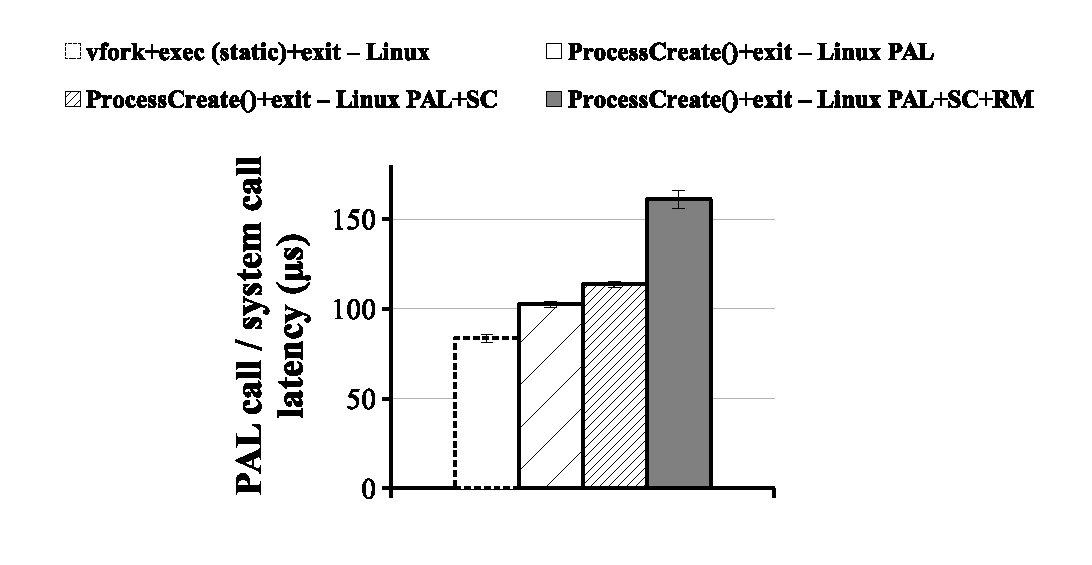
\includegraphics[height=10em]{proc-latency}
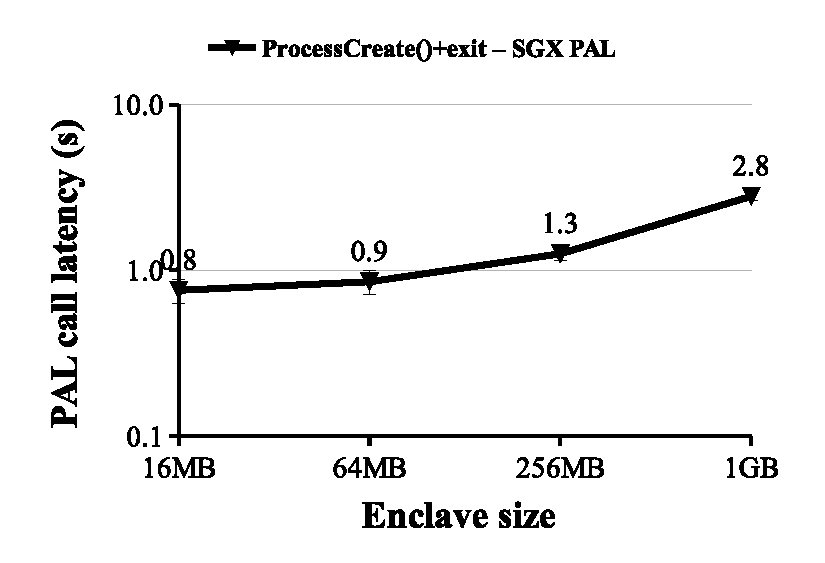
\includegraphics[height=10em]{sgx-proc-latency}
}
\parbox{0.59\textwidth}{\centering\bf (a) process creation+exit}
\parbox{0.39\textwidth}{\centering\bf (b) \sgx{} enclave creation+termination}
\caption{Latency of creating (a) a clean process on the Linux PAL, and (b) an enclave on the \sgx{} PAL, in respect of different enclave sizes.
The comparison is between (1) a combination of \syscall{vfork} and \syscall{exec} with a minimal static program on Linux; (2) \palcall{ProcessCreate} on the Linux PAL, with and without a \seccomp{} filter ({\bf +SC}) and reference monitor ({\bf +RM}); (3) the same \hostapi{} on the \sgx{} PAL.}
\label{fig:eval:pal:proc-latency}
\end{figure*}










%the latency of similar operations
%on a Linux kernel.
%The initialization time of the Linux PAL
%contributes a large portion to this overhead, besides the minor cost of establishing the RPC stream
%between the parent and child processes (using an unnamed UNIX domain socket).
%The Linux PAL
%with the \seccomp{} filter installed
%subjects to the same overheads,
%except in order to force the PAL binary always loaded
%at the same address,
%a separate security loader starts
%in each new process
%at a low, static address
%to load the PAL binary afterwards. 
%The overhead with the \seccomp{} filter installed
%is \roughly{}26\%,
%including the system call slowdown
%and the extra cost of reloading the PAL loader in each new process.
%If the reference monitor
%is enabled,
%the reference monitor
%must attach the new process to the sandbox
%inside the Linux kernel,
%and always check that the new process only loads the security loader instead of any other binaries.
%The overhead with both the \seccomp{} filter
%and the reference monitor
%is \roughly{}93\%.



\paragraph{Process creation on SGX.}
The \sgx{} PAL isolates each process inside a separate enclave
and uses secured RPC streams
for coordination between parent and child processes.
As a part of the process creation,
the \sgx{} PAL initializes an empty enclave
signed for the target executable
and establishes a TLS connection over an RPC stream.
The process creation procedure
includes several defenses against potential attacks
from the host OS,
including impersonating one of the enclaves and launching man-in-the-middle attacks on RPCs~\cite{shinde17panoply}.
%Enclave creation and
%security defenses %against these attacks
%cause the overheads
%observed on the \sgx{} PAL.
The \sgx{} PAL defends these attacks
using the local attestation feature of \sgx{} hardware and several cryptographic techniques.



Although establishing the TLS connections slows down
process creation,
the largest portion of process creation overheads
on the \sgx{} PAL
turns out to be enclave creation.
%as shown in Figure~\ref{fig:eval:pal:proc-latency} (b).
Figure~\ref{fig:eval:pal:proc-latency} (b)
evaluates the cost of enclave creation
by gradually increasing the enclave size of each new process.
The results show that
the process creation time on the \sgx{} PAL
is largely correlated with
enclave sizes;
%Since enclave sizes are irrelevant from
%the cost of defending against Iago attacks,
%enclave creation time
%is responsible of most overheads when a new process is created in a large enclave.
%completely subjects to enclave creation time.
%For the \sgx{} PAL,
%the latency of creating a new enclave for each child process
%is significantly higher
%than creating a normal \picoproc{}.
%Figure~\ref{fig:eval:pal:proc-latency} (b)
%shows that the latency of enclave creation
%is related, but not proportional,
%to the enclave size configured by users.
%To create a 16MB enclave,
%which is the minimum size to load a functioning \graphene{} process,
%takes \roughly{}0.8\asec{}.
creating a process in a 1GB enclave
takes \roughly{}2.8\asec{},
or 26,000\x{} to the process creation time
on the Linux PAL.
%and will cause significant slowdown
%to the guest if the guest frequently spawns processes.
%Although some techniques such as
%preallocating empty enclave may reduce
%the enclave creation time,
%this thesis leaves such experiment as future work.
%Furthermore,
%the \sgx{} version 2 hardware
%with support dynamic memory management,
%and eliminate the need of preserving large heap space in enclave
Although process creation
is normally considered an expensive operation
in most OSes,
the extremely high overheads
on the \sgx{} PAL
can be a huge impact, especially for applications which
frequently create new processes, such as shell applications and makefiles.


Several optimizations are possible for improving process creation
on the \sgx{} PAL.
One optimization
is to create enclaves in advance
or to recycle enclaves after process termination.
Moreover,
the SGX2 hardware~\cite{sgx2} introduces
new instructions for inserting empty pages into an enclave
after initialization,
and therefore allows new processes to start
in small enclaves.
%An ongoing extension of \graphene{}
%ports the \sgx{} PAL to the SGX2 hardware,
%and shows \roughly{}50\% reduction
%on total execution time of a ``hello world'' program.






\paragraph{Bulk IPC vs RPC streams.}
\Thehostabi{} introduces an optional, bulk IPC feature for improving RPC messaging.
The assumption around the
abstraction
is that it has higher bandwidth
than an RPC stream
by sharing pages as copy-on-write across processes.
However,
the assumption is not always valid, since RPC streams
can be as efficient as bulk IPC on some host OSes.
The concern is backed by the benchmark results in Figure~\ref{fig:eval:pal:gipc-bandwidth},
which show that
page-aligned RPC messaging on Linux kernels later than 4.2
is comparably efficient
as using the bulk IPC abstractions.
The reason is an optimization introduced on Linux 4.2
to implement zero-copy transfers
over UNIX sockets~\cite{linux4.2-unix}.
%The phenomenon
%is caused by an optimization introduced
%in Linux 4.2, which allows zero-copy transfer on UNIX domain sockets.
%is due to the introduction of a zero-copy design of UNIX domain sockets in 4.2.
%The zero-copy design
%allows a UNIX domain socket to share the physical pages
%of a page-aligned buffer
%with the destination process,
%creating the same effect as the bulk IPC feature in \thehostabi{}.
%Therefore, using the bulk IPC is only beneficial on a Linux kernel older than 4.2.
%Despite the optimization being less effective on latest Linux kernels,
\graphene{} still considers the bulk IPC abstraction
beneficial for older Linux kernels
or other host OSes. 



\begin{figure*}[t!]
\centering
\footnotesize
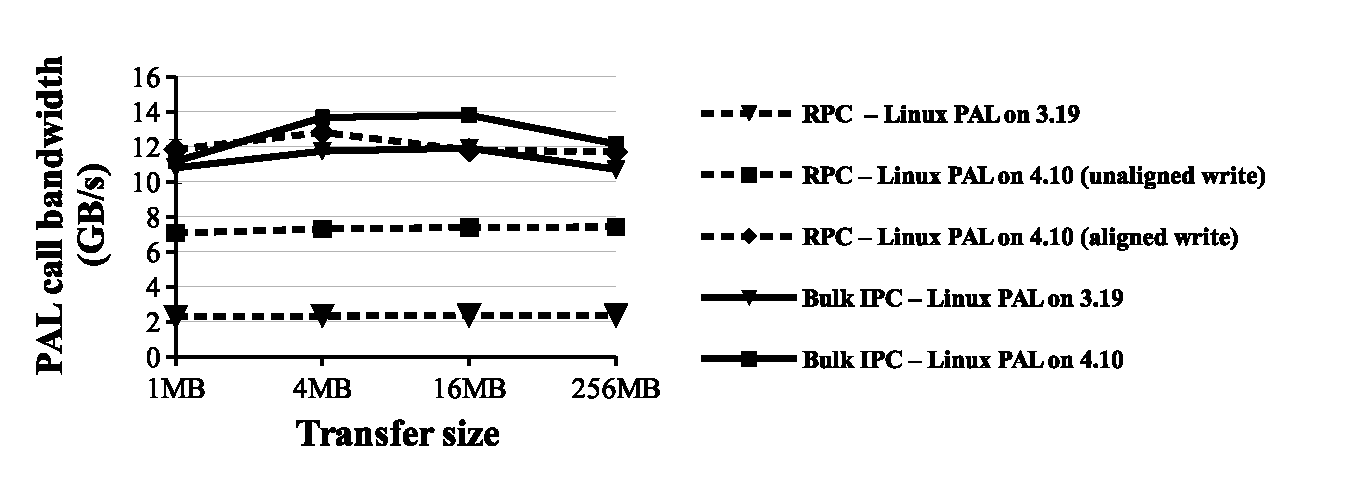
\includegraphics[width=.85\textwidth]{gipc-bandwidth}
\caption{Bandwidth of sending large messages over (a) RPC streams and (b) Bulk IPC channels. The messages are sent in different sizes (1MB to 256MB), and either aligned or unaligned with the page boundary.
Higher is better. Both abstractions are benchmarked on Linux kernel 3.19 and 4.10 as the hosts. The impact of the \seccomp{} filter or reference monitor is marginal (less than 1\%).}
\label{fig:eval:pal:gipc-bandwidth}
\end{figure*}


 




